\documentclass[1p]{elsarticle}

\usepackage{lineno,hyperref}
\modulolinenumbers[5]
\usepackage[utf8]{inputenc}
\usepackage[spanish]{babel}
\usepackage{amsmath}
\usepackage{graphicx}
\usepackage{amsfonts}
\usepackage{amssymb}
\newtheorem{thm}{Teorema}
\newtheorem{lem}[thm]{Lema}
\newdefinition{rmk}{Remark}
\newproof{pf}{Demostración}
\newproof{pot}{Demostración del Teorema \ref{thm2}}
%%\bibliographystyle{IEEEannot}

%% `Elsevier LaTeX' style
\bibliographystyle{elsarticle-num}
%%%%%%%%%%%%%%%%%%%%%%%
\usepackage{setspace}  
\begin{document}

\begin{frontmatter}

\title{Perspectives on mathematical modelling for Alhzeimer's disease}

%% Group authors per affiliation:
\author{Bartolomé Ortiz Viso}
\address{Master en Física y Matemáticas\\ Universidad de Granada\\17/01/2018}

\begin{abstract}
This work is a brief revision and study about some research articles related to Alhzeimer's disease (AD) published in last years. My aim is to present its mains results, some technical highlights related to the mathematical way of modelling the disease, and comment about its implications and future research. Althought this work is merely a revision it could be useful as a source of interesting models in cell dynamics and at a biomoleculal size dynamics due to the complexity of AD.
\end{abstract}

\begin{keyword}
 \texttt{Alhzeimer disease} \sep \texttt{cells dynamics}\sep \texttt{ordinary differential equations} \sep \texttt{partial differential equations}

\end{keyword}

\end{frontmatter}

\linenumbers

\section{Introducción}
\spacing{1.2}
La enfermedad de Alzheimer (EA) es una enfermedad neurodegenerativa progresiva que destruye la memoria y las habilidades cognitivas. Es una enfermedad muy común pero altamente destructiva a todos los niveles desde el puramente biológico al social. La EA tiene una gran tendencia a aparecer en personas de edades avanzadas, y las cifras entorno a ella no son nada alentadoras: Si no se encuentra una cura, para 2050, la cantidad de pacientes con Alzheimer
en los EE. UU. llegará a 15 millones y el costo de cuidarlos excederá  1 billón anualmente \cite{hao}
A pesar de lo que conocemos sobre la enfermedad hoy en día y de las investigaciones que se llevan a cabo, los mecanismos detrás del desarrollo de esta enfermedad siguen siendo un misterio.
Durante nuestro recorrido matemático se han escogido 4 artículos de referencia que, al estar en distintos periodos temporales modelan de una forma distinta la enfermedad centrándose en los conocimientos que se tenían en la época. Actualmente sabemos que la EA se caracteriza por la presencia de dos tipos de características neuropatológicas: placas extracelulares
que consiste en péptidos $\beta-$amiloides y marañas neurofibrilares intracelulares de proteínas tau-hiperfosforiladas.
Sin embargo actualmente no hay medicamento que pueda
curar, detiener o incluso ralentizar la progresión de la enfermedad. Esto se debe en gran parte a las conversaciones cruzadas complejas y dinámicas que se producen entre múltiples tipos de células en todo el proceso de envejecimiento.
A lo largo del trabajo presentaremos un pequeño esquema biológico global y luego presentaremos los modelos particulares, así como su motivación biológica y matemática particular.


\section{Esquema biológico global}
Con el fin de comprender a grandes rasgos qué sabemos sobre la enfermedad de Alhzeimer presentamos un breve esquema \ref{cerebro5} sobre lo que sabemos hasta ahora. Aportamos el dibujo de \cite{bibid} para apoyar visualmente los puntos centrales del esquema:
\begin{figure}
	\begin{center}
	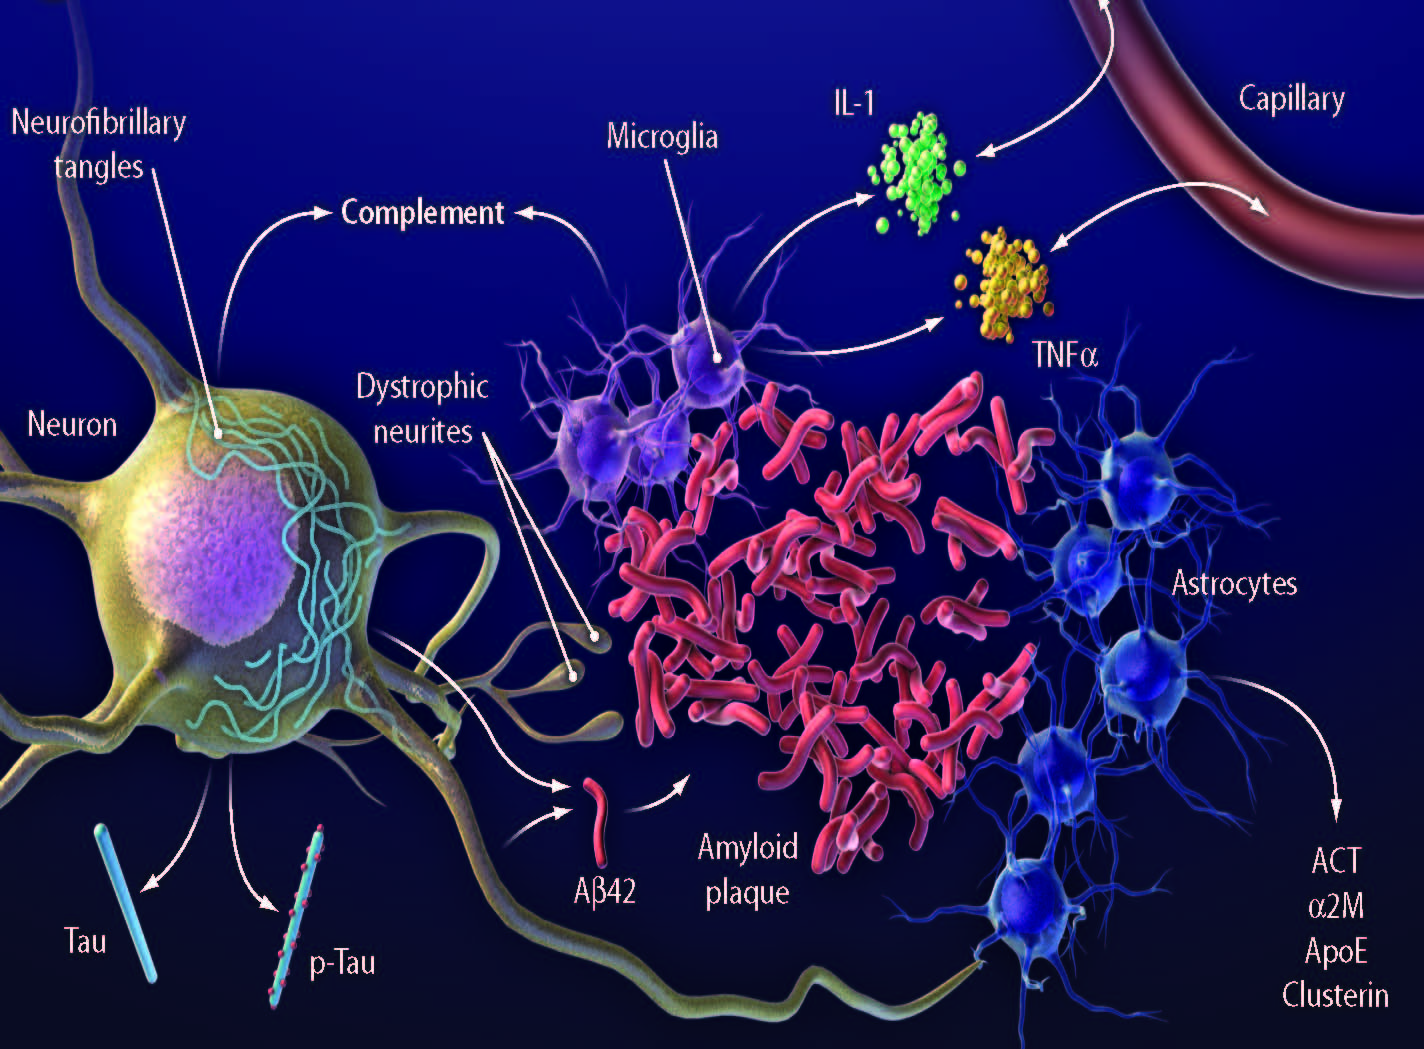
\includegraphics[scale=1]{imagen.jpg}
	\caption{Representacion esquemática del mecanismo biológico implicado}
	\label{cerebro5}
	\end{center}
\end{figure}
\begin{itemize}
	\item La enfermedad de Alzheimer se caracteriza por la aparicion de placas seniles (o placas amiloides) y ovillos neurofibrilares, y desemboca en una pérdida de neuronas y sinapsis en la corteza cerebral y en ciertas regiones subcorticales.
	\item Las placas son depósitos densos, insolubles, de la proteína beta-amiloide y de material celular que se localizan fuera y alrededor de las neuronas. Estas continúan creciendo hasta formar fibras entretejidas dentro de la célula nerviosa, los llamados ovillos.
	\item Recientemente también se ha incorporado el rol de la proteina tau: su aglomeración en fibras desintegra el sistema de transporte de la neurona. Así como el papel de la proteína APP de cuya proteolisis aprecerían los 
	conglomerado iniciales de proteína beta-amiloide
	\item Aunque no se sabe exactamente el papel que juegan las placas seniles, se sabe que la acumulación de las fibras amiloides es responsable de la perturbación de la homeostasis del ion calcio intracelular, lo que induce la muerte celular programada, llamada apoptosis.
	\item Varios mecanismos inflamatorios y la intervención de las citoquinas pueden también jugar un papel en la patología de la enfermedad de Alzheimer. La inflamación es el marcador general de daño en los tejidos en cualquier enfermedad y puede ser secundario al daño producido por el alzhéimer, o bien, la expresión de una respuesta inmunológica, algo que recogen muchos modelos a través de las poblaciones de la microglia (sistema inmune, macrófagos inmunes innatos residentes dentro de los tejidos del cerebro) y la astroglia.
\end{itemize}
\paragraph{Código representativo}

Como comentabamos en la introducción, durante el trabajo se exponen varios artículos. Durante el estudio del mismo se ha diseñado un pequeño código, que se aporta a continuacion y en el encabezado de los modelos, para discernir rápidamente las características que involucran en el desarrollo de ese modelo en particular:
 \begin{enumerate}
 	\item Poblaciones neuronales
 	\item Péptidos de Beta-Amiloide (Comportamiento priónico:A, Sin él:B)
 	\item Microglia
 	\item Astroglia
 	\item Proteínas $PPA$ y $PrP^C$
 	\item Escala temporal (única: A, combinación de varias: B)
 \end{enumerate}
Pasamos ya a tratar los modelos uno a uno, por orden cronológico. 

\section{1º Modelo: Patogénesis (1,2B,3,4,6B)}
Se trata del modelo que proponen \textit{Puri, Ishwar K $,$ Li, Liwu} en su articulo \textbf{Mathematical modeling for the pathogenesis of Alzheimer's disease}\cite{puri}. En este caso tratamos con un modelo que pretende abordar la enfermedad desde el punto de vista patogénico describiendo como se relacionan los gr$,$es grupos de celulas involucrado en la EA: Microglia (M1 y M2), Astroglia (Aq y Ap), Beta-Amiloide ($A\beta$) y la poblacion de Neuronas ($N_s$, $N_d$).


\subsection{Hipótesis de modelado} Partimos de las sugerencias presenciadas en estudios sobre como la microglia puede jugar un papel importante
durante el inicio y la progresión de la enfermedad. Microglia
es capaz de expresar caracter proinflamatorios y reactivos
especie de oxígeno cuando se activa por señales inflamatorias cuando aumenta el $A\beta$. En cerebros sanos, junto con quiescentes astroglia $Aq$, la microglía en reposo puede adoptar un estado antiinflamatorio  $M2$ y a su vez fomentar la supervivencia neuronal $Ns$ y prevenir
proliferación de astroglia proliferante $Ap$. Si aparecen esas señales como el $A\beta$ la microglia puede adoptar un estado proinflamatorio $M1$, lo que lleva a la proliferación de $A_p$ y la muerte neuronal $N_s$. Restos neuronales,$A\beta$ y / o la Ap a su vez puede exacerbar aún más la inflamación
de la microglia . El esquema final de las interacciones se puede ver en la figura \ref{cerebro12}

\begin{figure}
	\begin{center}
	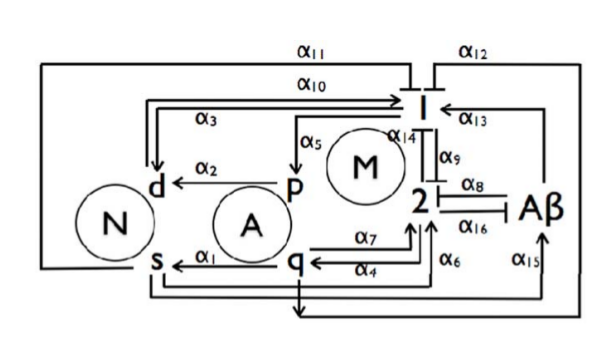
\includegraphics[scale=0.5]{primerdiagrama1.png}
	\caption{Representacion esquemática del mecanismo}
	\label{cerebro12}
		\end{center}
\end{figure}
\subsection{Modelo final}
Para modelar las interacciones se utiliza una ley de accion de masas clásica quedando el siguiente resultado:
\begin{equation}
\left\lbrace
\begin{array}{ll}
dN_s/dt=\alpha_1A_q-\alpha_2A_p-\alpha_3M_1 \\
dN_s/dt=-dN_d/dt\\
dA_q/dt=\alpha_4M_2-\alpha_5M_1 \\
-dA_q/dt=dA_p/dt \\
dM_2/dt=(\alpha_6+\alpha_{11})N_s-\alpha_{10}N_d-(\alpha_7+\alpha_{12})A_q-\alpha_9M_1\\+\alpha_{14}M_2-(\alpha_8+\alpha_{13})A\beta\\
dM_1/dt=-dM_2/dt \\
dA\beta/dt=\alpha_{15}N_s-\alpha_{16}M
\end{array}
\right.
\end{equation}

\subsection{Puntos a destacar}
Aunque el modelado mediante ley de accion de masas es consecuente, realmente no tenemos idea alguna sobre los parámetros del sistema. Es por ello que el estudio se centra en calcular unas cotas de la estabilidad numérica frente a variaciones de los parámetros y las condiciones iniciales. 

Constituye un interesante avance en su época y aun con las carencias que presenta el estudio es capaz de señalar la importancia de la microglia en el desarrollo de la enfermedad y a puntar al beta-amiloide como un posible target para el desarrollo de terapias.

Sin embargo, como decimos, muchos aspectos que hoy sabemos se dejan en el proceso de abstraccion. Entre ellos cabe destacar el comportamiento del beta-amiloide. Al ser señalado como principal target para las terapias, empiezan a desarrollarse artículos que estudian su comportamiento, como el siguiente de nuestra lista.






\section{2º Modelo:Comportamiento del $A\beta$ (1,2A,5,6A)}
Se trata del modelo que proponen \textit{Helal, Mohamed $,$ Hingant, Erwan $,$ Pujo-Menjouet, Laurent $,$ Webb, Glenn F.} en su articulo \textbf{Alzheimer’s disease: analysis of a mathematical model incorporating the role of prions} \cite{helal}. En este caso tratamos con un modelo que pretende abordar el mecanismo por el cual se generań las acumulaciones de beta-amiloide.

\subsection{Hipótesis de modelado} El modelo estudia la relacion entre cuatro especies diferentes. Primero, la concentración de oligómeros de $A\beta$
que consiste en agregados de unos pocos péptidos $A\beta$; segundo, la concentración de la Proteína PrP'C; tercero, la concentración del complejo formado a partir de un oligómero de $A\beta$
unión a una proteína PrP'C. Estas cantidades son solubles y su concentración se describirá en términos de ecuaciones diferenciales ordinarias. En cuarto lugar, tenemos las
placas $A\beta$ descritas por una densidad de acuerdo con su tamaño x. Este enfoque
es estándar en el modelado de fenómenos de proliferación de priones. Señalamos que el tamaño x es una variable abstracta que podría
ser el volumen del agregado. Aquí, sin embargo,se ven los agregados como fibrillas que se
alargan en una dimensión. La variable de tamaño x por lo tanto pertenece al intervalo $(x_0, +\infty)$,
donde $x_0\geq 0$ representa un tamaño crítico por debajo del cual las placas no pueden formarse. Tenemos por tanto $\forall t\geq0$:
\begin{itemize}
	\item  $f (t, x) \geq 0$: la densidad de las placas $A\beta$ de tamaño x en el tiempo t,
	\item   $u (t) \geq 0$: la concentración de oligómeros solubles de $A\beta$ (oligómeros ilimitados) en
	tiempo t,
	\item  $p (t) \geq 0$: la concentración de proteínas priónicas celulares PrP'C en el momento t,
	\item  $b (t) \geq 0$: la concentración del complejo $A\beta$-x-PrP'C (oligómeros acotados) en el tiempo t.
\end{itemize}

Tengamos en cuenta que las placas de $A\beta$ se forman a partir de la agrupación de oligómeros de $A\beta$.
La velocidad de aglomeración depende de la concentración de oligómeros solubles y la
estructura del amiloide está vinculada a su tamaño. 
Suponemos, de hecho, que la masa de un oligómero está dada por un parámetro "suficientemente pequeño"
 $\epsilon> 0$. Por lo tanto, el número de oligómeros en una placa de masa $x> 0$ es
$x / \epsilon$ que justifica nuestra suposición de que el tamaño de las placas es un continuo. Además,
los amiloides tienen un tamaño crítico $x_0 = \epsilon n> 0$.
 El esquema de las interacciones se puede ver en la figura \ref{cerebro5}

	\begin{figure}
		\begin{center}
		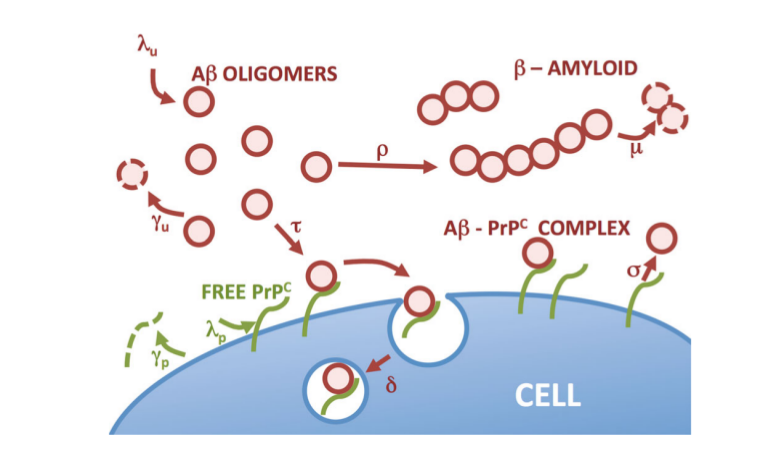
\includegraphics[scale=0.5]{segunda1.png}
		\caption{Representacion esquemática del mecanismo}
		\label{cerebro5}
			\end{center}
	\end{figure}

\subsection{Modelo final}

\begin{equation}
\left\lbrace
\begin{array}{ll}
\partial_tf(t,x)+u(t)\partial_x[\rho(x)f(t,x)]=\mu(x)f(x,t) \\
du/dt=\lambda_u-\gamma_u-\tau u p+\sigma b-nN(u)-\frac{1}{3}u\int_{x_0}^{\infty}p(x)f(x,t)dx\\
dp/dt=\lambda_p-\gamma_pp-\tau u p+\sigma b  \\
db/dt=\tau u p-(\sigma+\delta)b
\end{array}
\right.
\end{equation}
Destacamos la ecuación de evolución del primer término (donde $\rho(x)$ es la tasa de conversión de oligomeros en placa) y la integral en la segunda ecuacion, que representa el total de oligomeros que se unen formando polímeros.
\subsection{Puntos a destacar}
El estudio del articulo se centra en estudiar el buen planteamiento del problema y algunos resultados de su comportamiento.
EN primer lugar hay que destacar que debemos escoger un $\rho$ para comenzar el estudio de nuestro modelo. En el artículo se toman dos posibles respuestas:
no depende del tamaño de la placa o que dependa exponencialmente de esta. El primer caso es biologicamente poco realista pero más tratable analíticamente, el segundo conlleva un trabajo más pesado, aunque tiene mayor sentido biológico.
Dentro del trabajo destacamos algunos detalles que nos parecen de interés:
\begin{enumerate}
	\item La formación de polímeros es compleja e intervienen muchos procesos.
	\item No todo conjunto $A\beta$ es estable, sería necesaria la intervención de ecuaciones más precisas que describan de una manera más representativa este proceso.
	\item El resultado teórico en el primer caso expone una estabilidad ¿Es representativo? Se podría argumentar que dados los paso abstractivos que nos ha llevado a el, no posee una fuerza predictiva relevante.
\end{enumerate}
Con esta idea en mente, presentamos el tercer modelo.







\section{3º Modelo:Comportamiento prionico + difusión + Transporte (1,2A,5,6AB)}
Se trata del modelo que proponen \textit{Bertsch, Michiel $,$ Franchi, Bruno $,$ Marcello, Norina $,$ Tesi, Maria Carla $,$ Tosin, Andrea} en su articulo \textbf{Alzheimer's disease: a mathematical model for onset $,$ progression} \cite{bertsch}. En este caso tratamos con un modelo que pretende abordar el mecanismo por el cual se generań las acumulaciones de beta-amiloide y como se transmiten de neurona a neurona, junt$,$o mucha de la información disponible. El artículo además presenta gran cantidad de simulaciones numéricas, sin embargo en 2017 sus autores prueban el buen planteamiento del sistema.

\subsection{Hipótesis de modelado} El modelo presenta el comportamiento de las agregaciones de $A\beta$ mediante la ecuacion de difusion y le añade un termino que hemos visto en clase: ecuaciones de aglomeracion de Smoluchowski. Estas poblaciones vendrán determinadas por la longitud del polímero, e identificadas por $u_k$ con k la longitud.
Po otra parte el malfuncionamiento de la neurona viene determinado por el parametro a que puede variar en un rango de 0 a 1. Esto nos vale para definir una variable $f(t,x,a)$ que representa la cantidad de neuronas proximas a x que en tiempo t tienen un grado de malfuncionamiento a.
De f saldra además un término que indica como las neuronas dañadas producen $A\beta$ oligomeros y la propia fuente de estos fallos vendrá determinada por un funcionan que depende de una funcion de probabilidad, donde se engloba fallos geneticos que produzcan malfuncionamiento o saltos aletorios de manera que la enfermedad se extiende. 
Con ello tenemos dos grupos de variables (f y $u_k$) que pueden funcionar a tiempos distintos, por lo que se añade una escala temporal en el modelo final.

\subsection{Modelo final}

	\begin{equation}
	\left\lbrace
	\begin{array}{ll}
	\partial_tf+\partial_a(f\nu[f])=J[f] \\
	\epsilon\partial_tu_1=d_1\nabla^2u_1+[u_1\sum_{j=1}^{N}a_{1,j}u_j]+F[f]-\sigma_1u_1\\
	\epsilon\partial_tu_m=d_m\nabla^2u_m+[\frac{1}{2}\sum_{j=1}^{m-1}a_{j,m}u_ju_{m-j}-u_m\sum_{j=1}^{N}a_{m,j}u_j]  \\
	\epsilon\partial_tu_N=+\frac{1}{2}\sum_{j+k\geq N}a_{j,k}u_ju_k
	\end{array}
	\right.
	\end{equation}

\subsection{Puntos a destacar}
Es interesante como este modelo puede utilizarse para estudiar comportamientos en discretizaciones similares al cerebro, como se puede ver en la figura\ref{cerebro12} 
\begin{figure}
	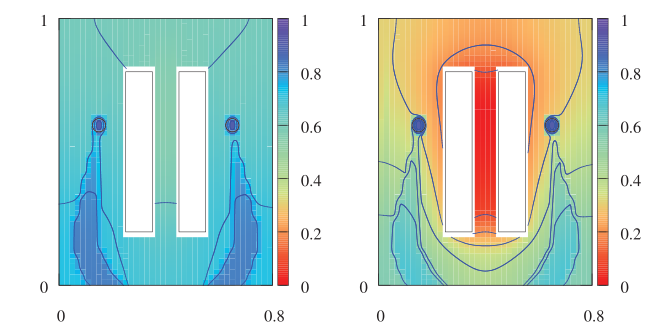
\includegraphics[scale=0.6]{tercer2.png}
	\caption{Expansión de malfuncionamiento neuronal en T=52 según la cantidad de $A\beta$. A la izquierda se puede observar como una cantidad mayor, provoca unos efectos devastadores (el degradado de colores representa la variable a)  }
	\label{cerebro12}
\end{figure}
También es interesante como se pueden estudiar en estos modelos la posible eficacia de medicamentos cuyo target es conocido, gracias a su orientacion en comprender la evolucion no solo de las sustancias si no de los biomarcadores. Se puede observar por ejemplo en la figura\ref{cerebro26}  
	\begin{figure}
		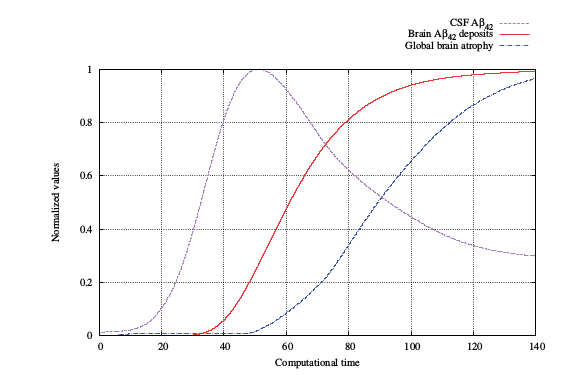
\includegraphics[scale=0.6]{tercer3.png}
		\caption{Evolución de los biomarcadores (CSF es el utilizado para medir el $A\beta$)}
		\label{cerebro26}
	\end{figure}
Con esta idea saltamos al ultimo modelo, objetivo: crear un sistema complejo que nos permita probar la eficacia teórica que pudieran tener los marcadores.

\section{4º Modelo:Comportamiento complejo total ( 1,2A,3,4,5,6B)}
Se trata del modelo que proponen \textit{Hao, Wenrui $,$ Friedman, Avner} en su articulo \textbf{Mathematical model on Alzheimer’s disease} \cite{hao}. En este caso tratamos con un modelo que pretende abordar el mecanismo de la EA desde un punto de vista global consider$,$o muchas variables que afectan en el desarrollo de la enfermedad.

\subsection{Hipótesis de modelado} 
El modelo presenta una estructura sencilla que involucra el movimiento de grupos celulares a través de la difusión y de la interacción de sustancias a traves de la ley de acción de masas. En este modelo, al componerse de 18 ecuaciones diferenciales acopladas, se pasa directamente a sus estudio numérico y se compara como disinttos medicamentos pueden influir en la enfermedad.  A continuación se muestran figuras ilustrativas para tal caso \ref{cerebro11}\ref{cerebro13}\ref{cerebro15}\ref{cerebro17}\ref{cerebro21}

	\begin{figure}
		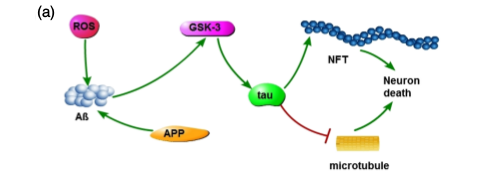
\includegraphics[scale=0.7]{primerdiagrama.png}
		\caption{Evolución del sistema biológico particular asociado a las rutas de APP}
		\label{cerebro11}
	\end{figure}

	\begin{figure}
		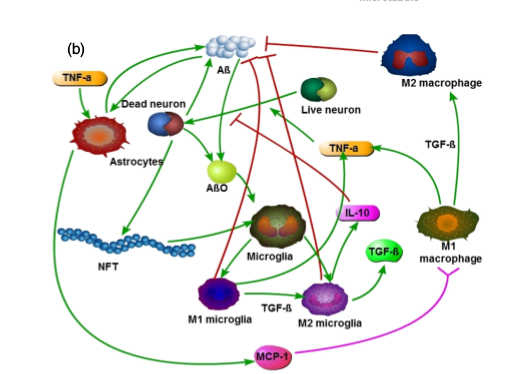
\includegraphics[scale=0.7]{segundodiagrama.png}
		\caption{Evolución del sistema biológico en general con todas las poblaciones posibles y las relaciones entre ellas }
		\label{cerebro13}
	\end{figure}

	\begin{figure}
		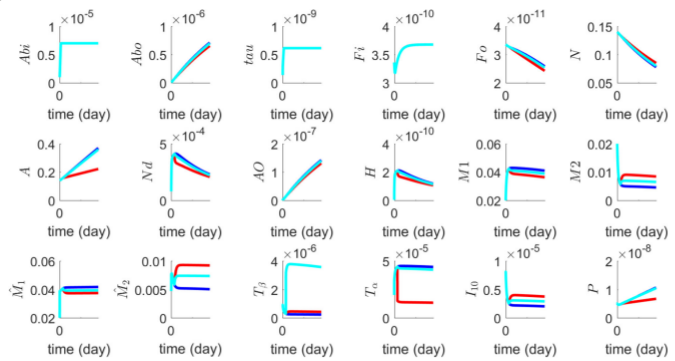
\includegraphics[scale=0.5]{cuarto.png}
		\caption{Evolución del sistema con tratamiento (rojo y azul claro) o sin el (azul oscuro)}
		\label{cerebro17}
	\end{figure}

	\begin{figure}
		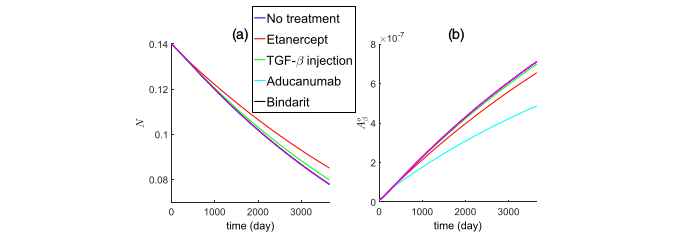
\includegraphics[scale=0.7]{quinto.png}
		\caption{Evolucion de la enfermedad con distintos tratamientos, se puede observar como tratamiento que afectan sobre la tasa de degradacion del $A\beta$ (rojo y azul claro) afectan positivamente frente a otros o a la ausencia del mismo}
		\label{cerebro21}
	\end{figure}

	\begin{figure}
		\begin{center}
		
		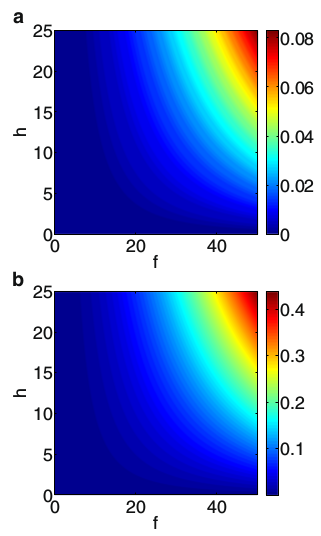
\includegraphics[scale=0.7]{sexta.png}
		\caption{Efectividad del tratamiento con la simulación, este proceso se calcula para hallar una dosis optima de varios tratamientos (h y f) y estudiar de que forma se complementan.}
		\label{cerebro15}
		
		\end{center}
	\end{figure}










\section*{Referencias}

\bibliography{bibliodinamica}

\end{document}